\documentclass{article}
\title{Beamforming for Telescope Array : 3D-FFT }
\author{Chenhui Niu}
\usepackage{graphicx}
\usepackage{amsmath}
\begin{document}
\maketitle
\section{Theory for 3-D FFT to make beam forming}
\subsection{Interferometer theory}
If we have a 1-D array with N antennas , and Each of them receive signal from zenith taking a drifting observe. We could get visibility by taking correlator of which multiply signals from each other:\\
\begin{align*}
V_{mn}(\nu) &= A_m(\nu) \cdot A_n^*(\nu) \\
 	   		&= I \cdot e^{2i \pi \nu t}_m\cdot e^{-2i \pi \nu (t +\tau )}_n\\
 	   		&= I \cdot e^{2i \pi \nu \tau }\\
 	   		&= I \cdot e^{2i \pi \nu d\cdot \cos\theta_{(t)} }\\ 	  	   				
\end{align*}

Where $\tau$ is time delay between two antenna element.If we see following image, $\tau = d \cdot \cos\theta$, and d is the distance of two antennas. If we using $u=\frac{d}{\lambda},l=\cos\theta$ , and take exact frequency $\nu$, The euqation above will become:\\
\begin{eqnarray}
V_{mn}=V_{u}(l) = I_{u}(l) \cdot e^{i2\pi ul}
\end{eqnarray}
This is a visibility for one direction at $\theta$ , If we want got the the intensity of whole sky , we need integral $4\pi$ :
\begin{eqnarray}
V(u) = \int_{4\pi} I_u(l)\cdot e^{i2\pi ul} d\Omega 
\end{eqnarray}
Equation (2) is a kind of Fourier Transform ,We could get the total intensity I with it's inverse FT.According(1)
\begin{eqnarray}
I_{mn}=I_u = V_{u}(l)\cdot e^{-i2\pi ul}
\end{eqnarray}
If we have N antennas, we will get a lot of baseline u:
\begin{eqnarray}
I(l)=\int V_l(u)\cdot e^{-i2\pi ul} du\\
I_{total}=\iint V_l(u)\cdot e^{-i2\pi ul} dud\Omega
\end{eqnarray}
\begin{figure}
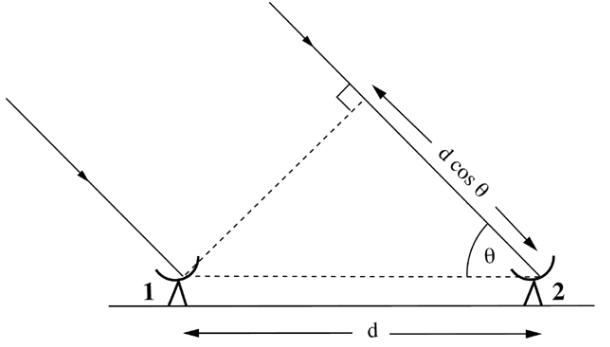
\includegraphics[width=\textwidth]{interferometer.png}
\caption{Interferometer for 2 antennas. d is the distance of 2 elements. source direction is at $\theta$.}
\end{figure}
\subsection{Beam forming}
In equation (5), We already got the intensity of whole sky. However,It's only a approximation In reality, It's hard to get the whole sky map because of the beam size of telescope. The telescope array only can change the beam resolution, The outlet of whole beam is depend on the single antenna. In general , it's not so large. If we want get the larger sky survey. we'd better to utilize the character of phase array to make larger survey. This step we called beam forming. \\

When we looking at each array element, and assume the beam is point on zenith, we could get the total beam direction of array. The signal for present is a summation of all the Intensity of all elements. If we want the total beam point slightly in a $\delta\theta$ of zenith, we could shift phases on partially elements. Further telescope need shift more, central element don't need to shift.  \\
If we discrete observe angle in equation (5):

\begin{eqnarray}\begin{aligned}
I_{total} &=\sum_u\sum_lV_l(u)\cdot e^{-i2\pi ul} \\
&=\sum_l(V_{11}(l)e^{-i2\pi ul}+V_{12}(l)e^{-i2\pi ul}+V_{13}(l)e^{-i2\pi ul}+\cdots)
\end{aligned}\end{eqnarray}
\begin{figure}
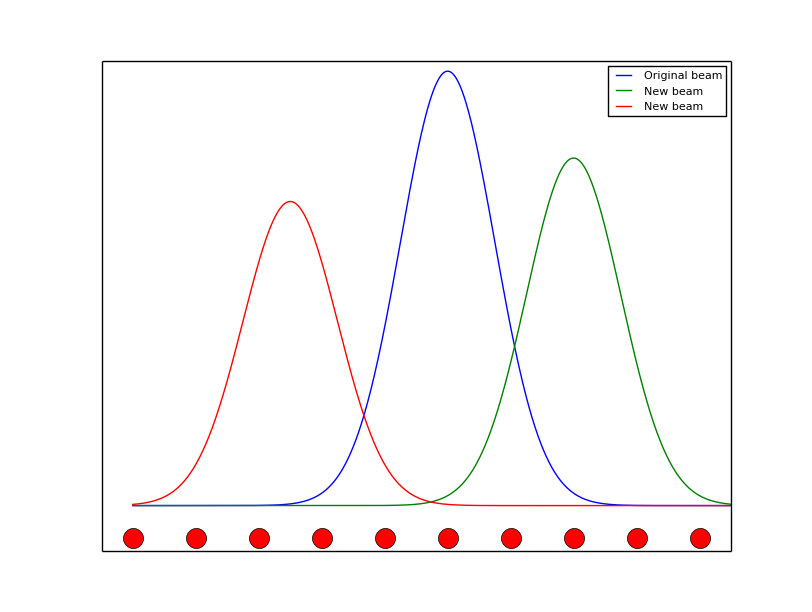
\includegraphics[scale=0.5]{beam.png}
\caption{red dot is represent antenna, Here we assume they are in a 1-D line. the blue one is the original beam, red and green is a new beam we form.}
\end{figure}
At one new formed beam, different antenna element has different phase shift factor. Assume at Beam i, antenna j has a shift factor $e^{-i2\pi\phi_j^i}$, we could get:
\begin{equation}
\begin{aligned}
\left\{ \begin{aligned}
 &I_1e^{-i2\pi\phi_1^1}&+&I_2e^{-i2\pi\phi_2^1}&+I_3e^{-i2\pi\phi_3^1}+\cdots+&I_je^{-i2\pi\phi_j^1}&,B_1&\\ 
 &I_1e^{-i2\pi\phi_1^2}&+&I_2e^{-i2\pi\phi_2^2}&+I_3e^{-i2\pi\phi_3^2}+\cdots+&I_je^{-i2\pi\phi_j^2}&,B_2&\\
 &\vdots& &\cdots\cdots& &\vdots&\vdots &&\\ 
 &I_1e^{-i2\pi\phi_1^i}&+&I_2e^{-i2\pi\phi_2^i}&+I_3e^{-i2\pi\phi_3^i}+\cdots+&I_je^{-i2\pi\phi_j^i}&,B_i&
 \end{aligned}\right.\\
\end{aligned}
\end{equation}
If we want total intensity of sky, we should sum all the beam together, we could do a FFT along the vertical direction of equation(7), then do a FFT along horizontal direction with variable u which is baseline.Then if we have a 2  dimensional telescope array, the beam forming could achieve by 3-D FFT.\\
There is a link between using Visibility to get $I_{total}$ and this method. If we change intensity of each element into amplitude or voltage, then in equations (7),it becomes:
\begin{equation}
I^i=(v_1e^{-i2\pi\phi_1^i}+v_2e^{-i2\pi\phi_2^i}+v_3e^{-i2\pi\phi_3^i}+\cdots+v_je^{-i2\pi\phi_j^i})^2
\end{equation}
Make a expansion, the complex voltage multiply will become the cross items. if we consider all beams , they will equal to the Visibility equation (6).
\subsection{Array shape}
As the science goal demand , the shape of Array might not be regular. This might caught the problem of FFT. To forbidden that, we often padding the array to uniform with zeros.See Figure 3.\\
\begin{figure}
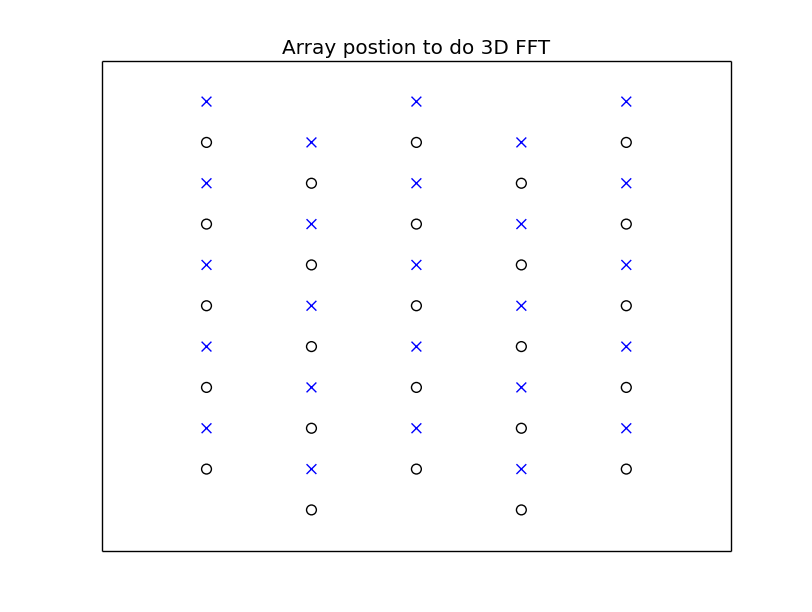
\includegraphics[width=\textwidth]{array_postion_to_3DFFT_beamforming.png}
\caption{Array might not distribute at regular shape, For get rid of this , we pad zeros between antennas to make it easier for FFT. ($\circ$) means the original antenna distribution, ($\times$) means padding position.}
\end{figure}

\section{Question}
I am not sure if this thinking is right, If we get the beam forming, should we get the whole Intensity of the sky? I think it might be good to have intensity of each beam. If so ,How is 3-D FFT to make a beam forming?

\end{document}